
編譯器優化對於高性能實現也很重要。運行一個編譯時根本沒有優化的程序,就能體會到編譯器的作用,一個未優化的程序(優化級別為0)運行速度比啟用所有優化後編譯的程序慢一個數量級。

然而,優化器可以從開發者那裡得到一些幫助。這種幫助可以通過非常微妙的形式,有時是反直覺的。在研究一些改進代碼優化的技術之前,有助於理解編譯器是如何處理程序的。

\subsubsubsection{10.2.1\hspace{0.2cm}編譯器優化的基礎知識}

關於優化必須瞭解的是,代碼都必須保持正確。這裡的正確與否與開發者主觀認為什麼是正確無關。程序可能會有錯誤,並給出一個看起來錯誤的答案,但編譯器必須保留這個答案,而定義不明確或調用未定義行為的程序則是例外。如果程序在標準看來是錯誤的,編譯器可以自由地做它想做的事情。我們將在下一章中來研究這一點。現在,我們將假設程序定義良好,並且只使用有效的C++語句。當然,由於答案不能因輸入組合而改變,所以編譯器在更改方面會受到限制。開發者可能知道某個輸入值是正的,或者某個字符串中的字符永遠不會超過16個,但編譯器並不知道(除非找到一種方法來告訴它)。編譯器只能夠證明這種轉換會產生完全等價的程序時,才能進行優化轉換,從而該程序對任何輸入都產生相同的輸出。實際中,若是複雜性讓編譯器難以控制,編譯器也會放棄修改。

理解這些是通過代碼成功地與編譯器交互,並實現更好的優化的關鍵。本章的其餘部分展示了不同的方法,可以證明某些理想的優化並不會改變程序的行為。

編譯器還受限於程序的信息。它只能處理編譯時已知的內容,不瞭解任何運行時數據,並且假設運行時的合法狀態都有可能。

下面是一個簡單的例子:

\begin{lstlisting}[style=styleCXX]
std::vector<int> v;
… fill v with data … 
for (int& x : v) ++x;
\end{lstlisting}

關注的焦點是最後一行——循環。如果手動展開循環,性能可能會更好,每個增量都有一個分支(循環終止條件),展開循環可以減少此開銷。在一個只有兩個元素的簡單\texttt{vector}例子中,最好完全刪除循環,只對兩個元素進行遞增。但是,\texttt{vector}的大小是運行時的信息,編譯器可能會生成一個帶有一些分支的部分展開循環來處理所有可能的\texttt{vector}大小,但它無法針對特定大小對代碼進行優化。

將它與下面的代碼進行對比:

\begin{lstlisting}[style=styleCXX]
int v[16];
… fill v with data … 
for (int& x : v) ++x;
\end{lstlisting}

現在編譯器確切地知道在循環中處理了多少整數,可以展開循環,甚至可以用一次操作多個數字的向量指令替換單個整數遞增操作(例如,在x86上的AVX2指令可以一次處理8個整數)。 

如果開發者知道\texttt{vector}總是有16個元素呢?可能並不重要。重要的是編譯器是否知道,並且能夠確定無誤,這比想象的要難。例如,以下代碼:

\begin{lstlisting}[style=styleCXX]
constexpr size_t N = 16;
std::vector<int> v(N);
… fill v with data … 
for (int& x : v) ++x;
\end{lstlisting}

開發者用他們自己的方式使\texttt{vector}的大小成為一個編譯時常量。編譯器會優化循環嗎?有可能。這完全取決於編譯器能否確定\texttt{vector}的大小不會改變。它將如何改變?可以先問問自己,填充\texttt{vector}的代碼中可能隱藏著什麼?雖然對於開發者來說這是已知的,但如何讓編譯器也知道呢?所有的代碼都是在構造和遞增循環這兩行之間編寫的,編譯器可以知道所有的東西(實際上,如果這個代碼段太長,編譯器就會放棄,並假設任何可能性,否則編譯時間就會爆炸)。但若調用一個函數,而該函數可以訪問\texttt{vector}對象,編譯器則無法知道該函數是否改變了\texttt{vector}的大小(除非該函數是內聯的)。像\texttt{fill\_vector\_without\_resizing()}這樣的函數名,只對開發者閱讀程序有幫助。 

即使沒有函數以\texttt{v}作為參數,仍然不清楚函數要如何訪問\texttt{vector}對象?如果\texttt{vector v}是在函數作用域中聲明的局部變量,那可能不能。但如果\texttt{v}是一個全局變量,任何函數都可以訪問它。類似地,如果\texttt{v}是類的成員變量,成員函數或友元函數都可以訪問它。因此,如果調用一個非內聯函數,這個函數不能通過參數直接訪問\texttt{v},那麼可以通過其他方式訪問\texttt{v}(並且對於創建局部變量的全局指針這一邪惡的做法,知道的人越少越好)。 

從開發者的角度來看,很容易高估編譯器所知道的東西。另外,在大多數情況下,把問題弄清楚並不是編譯器的優點。例如:可以在循環之前添加一個斷言:

\begin{lstlisting}[style=styleCXX]
constexpr size_t N = 16;
std::vector<int> v(N);
… fill v with data … 
assert(v.size() == N); // if (v.size() != N) abort();
for (int& x : v) ++x;
\end{lstlisting}

一些編譯器在使用最高的優化級別和未優化的上下文中,會推斷執行流不能進入循環,除非\texttt{vector}恰好有16個元素,並將優化該大小。並且,多數編譯器不會這麼做。

已經考慮過的基本示例中,用來幫助編譯器優化代碼的關鍵技術:

\begin{itemize}
\item
非內聯函數會破壞大多數優化,因為編譯器必須假設一個函數,但沒有看到具體的代碼,所以可以做任何合法的事情。 

\item
全局變量和共享變量對於優化有害。

\item
編譯器更可能優化短而簡單的代碼,而不是長而複雜的代碼。
	
\end{itemize}

第一個和最後一個在某種程度上有衝突。編譯器中的大多數優化都侷限於\textbf{基本代碼塊},這些塊只有一個入口點和一個出口點,在程序的流控制圖中充當節點。基本塊之所以重要,是因為編譯器可以看到塊內發生的一切,因此可以對不改變輸出的代碼轉換進行推理,所以內聯的優點是它增加了基本塊的大小。編譯器不知道非內聯函數在做什麼,所以需要做最壞的假設。但若函數是內聯的,編譯器就能確切地知道它在做什麼了(更重要的是,它沒有做什麼)。內聯的缺點也在於它增加了基本塊的大小,編譯器只能分析這麼多代碼,而不會使編譯時間變得不合理。內聯對於編譯器優化是非常重要的,原因我們將在後面進行討論。

\subsubsubsection{10.2.2\hspace{0.2cm}函數內聯}

當使用函數體的副本替換函數調用時,將由編譯器執行。為了實現這一點,內聯函數的定義必須在調用代碼的編譯過程中可見,調用的函數必須在編譯時已知。第一個要求在進行全程序優化的編譯器中是寬鬆的(不常見)。第二個要求排除虛函數調用和通過函數指針間接調用,並不是每個可以內聯的函數最終都可以內聯,編譯器必須權衡代碼膨脹和內聯帶來的好處。不同的編譯器對於內聯有不同的處理方法,C++的\texttt{inline}關鍵字只是一個建議,編譯器可以忽視。

函數調用內聯最明顯的好處是消除了函數調用的成本。大多數情況下,當函數調用的開銷不是那麼大,也就不重要了。其主要的好處是,編譯器跨函數調用的優化能力非常有限。考慮下面的代碼:

\begin{lstlisting}[style=styleCXX]
double f(int& i, double x) {
	double res = g(x);
	++i;
	res += h(x);
	res += g(x);
	++i;
	res += h(x);
	return res;
}
\end{lstlisting}

以下是有效的優化嗎?

\begin{lstlisting}[style=styleCXX]
double f(int& i, double x) {
	i += 2;
	return 2*(g(x) + h(x));
}
\end{lstlisting}

如果回答“是”,那麼仍然是從開發者的角度,而不是從編譯器的角度來看待這個問題。這種優化有很多方式會破壞代碼(對於編寫的合理的程序來說,可能沒有一種是正確的,但編譯器不能做的假設是自己是一個開發者)。 

\begin{itemize}
\item
首先,\texttt{g()}和\texttt{h()}可以產生輸出。這種情況下,消除重複的函數調用將改變可觀察行為。 

\item
其次,對\texttt{g()}的調用可能會鎖定一些互斥對象,而對\texttt{h()}的調用可能會解鎖它。這樣,執行的順序——調用\texttt{g()}鎖定,增加\texttt{i}計數,調用\texttt{h()}解鎖——就非常重要了。 

\item
第三,即使參數相同,\texttt{g()}和\texttt{h()}的結果也可能不同,例如:可以在內部使用隨機數。 

\item
最後(這種可能性經常被忽略),變量\texttt{i}是通過引用傳遞的,所以不知道調用者還對它做了什麼。可以是一個全局變量,或者某個對象可能會存儲對它的引用,函數\texttt{g()}和\texttt{h()}可能會對\texttt{i}進行操作,即使沒有看到它傳入到這些函數中。 
	
\end{itemize}

另一方面,如果函數\texttt{g()}和\texttt{h()}內聯,編譯器可以確切地看到發生了什麼:

\begin{lstlisting}[style=styleCXX]
double f(int& i, double x) {
	double res = x + 1; // g(x);
	++i;
	res += x – 1; // h(x);
	res += x + 1; // g(x)
	++i;
	res += x – 1; // h(x);
	return res;
}
\end{lstlisting}

整個函數\texttt{f()}現在是一個基本塊,編譯器只有一個限制:保留返回值。現在,就是一個有效的優化了:

\begin{lstlisting}[style=styleCXX]
double f(int& i, double x) {
	i += 2;
	return 4*x;
}
\end{lstlisting}

內聯對優化的影響可以延伸到很遠。考慮STL容器的析構函數,例如\texttt{std::vector<T>}。必須做的是調用容器中所有對象的析構函數:

\begin{lstlisting}[style=styleCXX]
for (auto it = crbegin(); it != crend(); ++it) it->~T();
\end{lstlisting}

因此,析構函數的執行時間與\texttt{vector}的大小N成正比。考慮一個由整數組成的\texttt{rstd::vector<int>},編譯器非常清楚析構函數在這種情況下的作用:什麼都不做。編譯器還可以看到,對\texttt{crbegin()}和\texttt{crend()}的調用並不會修改\texttt{vector}對象(如果想通過\texttt{const\_iterator}銷燬對象,請考慮如何銷燬\texttt{const}對象)。因此,可以消除整個循環。

現在考慮使用結構體的\texttt{vector}:

\begin{lstlisting}[style=styleCXX]
struct S {
	long a;
	double x;
};
std::vector<S> v;
\end{lstlisting}

這一次,類型\texttt{T}有一個析構函數,並且編譯器知道它的作用(因為通過編譯器生成)。同樣,析構函數什麼也不做,整個銷燬循環消除。對於默認析構函數也是如此:

\begin{lstlisting}[style=styleCXX]
struct S {
	long a;
	double x;
	~S() = default;
};
\end{lstlisting}

編譯器應該能夠為空析構函數做同樣的優化,但只有內聯時才會這麼做:

\begin{lstlisting}[style=styleCXX]
struct S {
	long a;
	double x;
	~S() {}     // Probably optimized away
};
\end{lstlisting}

另一方面,如果類聲明只是像下面這樣聲明析構函數:

\begin{lstlisting}[style=styleCXX]
struct S {
	long a;
	double x;
	~S();
};
\end{lstlisting}

定義是在單獨的編譯單元中提供的,然後編譯器為每個\texttt{vector}元素生成一個函數調用。這個函數仍然什麼也不做,但需要時間來運行循環,並執行N個函數調用。內聯允許編譯器將這優化為零。

這是內聯及其對優化的影響的關鍵,內聯允許編譯器看到在本來神祕的函數中沒有發生的事情。內聯還有另一個重要的作用,創建內聯函數體的唯一副本,可以使用調用者給出的特定輸入進行優化。在這個唯一的副本中,可能會觀察到一些對優化友好的條件,而這些條件對於函數通常是不正確的。下面是一個例子:

\begin{lstlisting}[style=styleCXX]
bool pred(int i) { return i == 0; }
… 
std::vector<int> v = … fill vector with data …;
auto it = std::find_if(v.begin(), v.end(), pred);
\end{lstlisting}

假設函數\texttt{pred()}的定義與對\texttt{std::find\_if()}的調用在同一個編譯單元中,對\texttt{pred()}的調用是否內聯?答案是“可能”,這主要取決於\texttt{find\_if()}是否內聯。現在,\texttt{find\_if()}是模板,所以編譯器可以看到函數的定義。如果\texttt{find\_if()}沒有內聯,則從模板中會為特定類型生成一個函數。這個函數中,第三個實參的類型是已知的:\texttt{bool (*)(int)}指向接受\texttt{int}類型並返回\texttt{bool}類型的函數的指針。但是這個指針在編譯時未知,同一個\texttt{find\_if()}函數可以用許多不同的謂詞來調用,這些謂詞都不能是內聯的。只有當編譯器為這個特定的調用生成唯一的\texttt{find\_if()}副本時,謂詞函數才能內聯。編譯器有時會這樣做,這就是所謂的複製。但在大多數情況下,內聯謂詞或作為參數傳入的其他內部函數的唯一方法,是首先內聯外部函數。 

這個特殊的例子在不同的編譯器上會產生不同的結果,GCC將只在最高的優化級別下內聯\texttt{find\_if()}和\texttt{pred()}。其他編譯器甚至不會這樣做。然而,還有另一種方法鼓勵編譯器使用內聯函數調用的方式,這似乎是反直覺的,因為這會向程序中添加了更多的代碼,並使嵌套函數調用更加冗長:

\begin{lstlisting}[style=styleCXX]
bool pred(int i) { return i == 0; }
… 
std::vector<int> v = … fill vector with data …;
auto it = std::find_if(v.begin(), v.end(), 
  [&](int i) { return pred(i); });
\end{lstlisting}

這裡的矛盾之處是,在同一個間接函數調用周圍添加了一個間接層,即Lambda表達式(假設開發者不想簡單地將謂詞直接複製到Lambda中有其他的原因)。即使編譯器沒有內聯\texttt{find\_if()},但\texttt{pred()}實際上更容易內聯。因為,這一次謂詞的類型是唯一的:每個Lambda表達式都有一個唯一的類型,因此對於這些特定的類型參數,\texttt{find\_if()}模板實例化一次。編譯器可能會內聯一個調用一次的函數,這樣做就不會生成過多的代碼。使對\texttt{find\_if()}的調用沒有內聯,但在該函數中,第三個參數只有一個可能,這個值在編譯時就知道是\texttt{pred()}。因此,對\texttt{pred()}的調用可以內聯。

現在,可以繼續在第1章中提出的“虛函數調用的成本”問題了。首先,編譯器使用函數指針表來實現虛調用,因此調用本身涉及到間接層。與非虛調用相比,CPU必須多讀一個指針,並多做一次跳轉。這為函數調用增加了更多的指令,使函數調用的代碼開銷增加了一倍(根據硬件和緩存狀態有很大的變化)。然而,我們通常調用一個函數來完成工作,因此函數調用的機制只是函數執行總時間的一部分。即使對於簡單函數,虛函數的開銷也很少超過非虛函數的10-15\%。

然而,在花費太多時間計算指令之前,應該質疑最初的問題的有效性。如果一個非虛函數調用是充分的,也就在編譯時就知道將調用哪個函數,為什麼一開始要使用虛函數呢?如果發現只在運行時調用哪個函數,就根本不能使用非虛函數,因此它的速度無關緊要。按照這個邏輯,應該比較虛函數調用和函數等價的運行時解決方案,有條件地調用幾個函數中的一個,使用一些運行時信息來選擇。使用\texttt{if-else}或\texttt{switch}通常會導致執行速度變慢,至少在要調用函數有兩個以上的重載版本時是這樣。最有效的實現是使用函數指針表,這正是編譯器對虛函數所做的。

當然,問題也並不是毫無意義。如果有一個帶有虛函數的多態類,但是在某些情況下,在編譯時就知道了實際的類型,該怎麼辦?這時,比較虛函數調用和非虛函數調用就有意義了。

還需要了解一下合適的編譯器優化。如果編譯器能夠在編譯時確定對象的真實類型,從而知道將調用虛擬函數的哪個重載版本,那麼它將在去虛擬化中將調用轉換為非虛的。

但是,為什麼要在討論內聯的章節中討論這個問題呢?因為我們忽略了一個事實,虛函數對性能的最大影響是(除非編譯器可以反虛化調用)不能內聯。一個簡單的函數,如\texttt{int f() {return x;}}的結果是在內聯之後只有一條,甚至沒有指令,但是非內聯版本具有常規的函數調用機制,就要慢一個數量級。若沒有內聯,編譯器就無法知道虛函數內部發生了什麼,必須對每一個外部可訪問的數據塊做出最壞的假設。所以在最壞的情況下,虛函數調用的代價可能會高出數千倍。

內聯、展示函數體實現和創建唯一的、特化的函數副本的兩種效果都有助於優化器,因為它們增加了編譯器對代碼的瞭解。若想幫助編譯器更好地優化代碼,那麼理解編譯器真正瞭解什麼非常重要。 

現在,我們將探討編譯器在不同的約束下運行的情況,這樣就可以發現錯誤的約束:一些是開發者認為是已知的,但編譯器卻不這麼認為的情況。 

\subsubsubsection{10.2.3\hspace{0.2cm}編譯器到底知道什麼?}

也許對優化的最大限制是,瞭解在此代碼執行期間可能會進行修改的內容。為什麼這很重要?下面是一個例子:

\begin{lstlisting}[style=styleCXX]
int g(int a);
int f(const std::vector<int>& v, bool b) {
	int sum = 0;
	for (int a : v) {
		if (b) sum += g(a);
	}
	return sum;
} 
\end{lstlisting}

只有\texttt{g()}的聲明是可用的。編譯器能優化\texttt{if()}語句,並消除條件的重複求值嗎?在經歷了本章所有的驚喜和陷阱之後,我們可能正在尋找一個不這樣做的原因。但結果是沒有,這是一個完全有效的優化:

\begin{lstlisting}[style=styleCXX]
int f(const std::vector<int>& v, bool b) {
	if (!b) return 0;
	int sum = 0;
	for (int a : v) {
		sum += g(a);
	}
	return sum;
} 

\end{lstlisting}

現在讓稍微修改一下這個例子:

\begin{lstlisting}[style=styleCXX]
int g(int a);
int f(const std::vector<int>& v, const bool& b) {
	int sum = 0;
	for (int a : v) {
		if (b) sum += g(a);
	}
	return sum;
} 
\end{lstlisting}

為什麼要通過\texttt{const}引用傳遞\texttt{bool}形參呢?最常見的原因是模板。如果有一個模板函數不需要複製實參,則必須聲明形參為\texttt{const T\&},這裡假設\texttt{T}可以是任何類型。如果\texttt{T}推斷為\texttt{bool}類型,那麼現在就有了一個\texttt{const bool\&}形參。這裡的變化可能很小,但對優化的影響是深遠的。如果還認為之前所做的優化有效,請在更大的上下文中考慮我們的示例。現在可以看到所有內容(假設編譯器仍然不可見):

\begin{lstlisting}[style=styleCXX]
bool flag = false;
int g(int a) {
	flag = a == 0;
	return –a;
}
int f(const std::vector<int>& v, const bool& b) {
	int sum = 0;
	for (int a : v) {
		if (b) sum += g(a);
	}
	return sum;
} 
int main() {
	f({0, 1, 2, 3, 4}, flag);
}
\end{lstlisting}

通過調用\texttt{g()},可以改變\texttt{b},因為\texttt{b}是一個綁定到全局變量的引用,該全局變量也可以在\texttt{g()}中訪問。在第一次迭代中,\texttt{b}為false,但是對\texttt{g()}的調用有一個副作用,\texttt{b}變為了true。如果參數按值傳遞,則不會發生這種情況。值在函數最開始捕獲,並且不跟蹤調用者的變量。但是通過引用傳遞,並且循環的第二次迭代不再是固定的代碼。每次迭代中,必須計算條件,並且不可能進行優化。再次強調,“開發者知道的”和“編譯器知道的”之間的區別是,代碼中沒有全局變量,或者確切地知道函數\texttt{g()}的作用。編譯器不能做出這樣的猜測,並且必須假設程序做了(或在將來的某個時候會做)類似於前面的例子中演示的事情,這使得優化可能不安全。 

如果函數\texttt{g()}是內聯的,並且編譯器知道它沒有修改全局變量,那麼這種情況就不會發生。但不能期望所有代碼都內聯,因此在某些情況下,必須考慮如何幫助編譯器確定它不知道的內容。當前的示例中,最簡單的方法是引入一個臨時變量(當然,在這個簡單的示例中,可以手工進行優化,但這在更復雜的實際代碼中並不實用)。為了讓這個例子更真實一點,要記住函數\texttt{f()}可能來自一個模板的實例化。我們不想對未知類型的形參\texttt{b}進行復制,但知道它必須可以轉換為\texttt{bool}類型,因此\texttt{bool}類型可以作為臨時變量的類型:

\begin{lstlisting}[style=styleCXX]
template <typename T>
int f(const std::vector<int>& v, const T& t) {
	const bool b = bool(t);
	int sum = 0;
	for (int a: v) {
		if (b) sum += g(a);
	}
	return sum;
}
\end{lstlisting}

編譯器仍然假設函數\texttt{g()}可能會改變\texttt{t}的值。但這不再重要,條件使用了臨時變量\texttt{b},絕對不能改變,因為在函數\texttt{f()}之外不可見。當然,如果函數\texttt{g()}可以訪問,並改變\texttt{f()}第二個參數的全局變量,那麼轉換就改變了程序的結果。通過創建這個臨時變量,告訴編譯器這種情況不會發生。這是編譯器自己無法獲得的信息。 

這很容易理解,但在實踐中相當困難。若已知一些東西,但編譯器不可能知道,就需要以一種編譯器可以使用的方式進行斷言。這很難做到的原因是,我們通常不會像編譯器那樣思考,而且很難放棄自己知道絕對正確的假設。 

這裡把臨時變量\texttt{b}聲明為\texttt{const}了嗎?這主要是為避免因意外修改而產生的錯誤,但這也有助於編譯器。編譯器能夠看到沒有改變\texttt{b}。與前面複雜的情況不同,編譯器看到了對\texttt{b}的所有操作。然而,不能僅因為這些是可用的就確定編譯器一定了解。分析程序需要時間,開發者只願意等待編譯器完成它的工作。另一方面,語法檢查是必須的。如果聲明變量\texttt{const}並試圖修改,程序將無法編譯,將不會進入優化步驟。因此,優化器可以假設\texttt{const}變量都不會改變。在可能的情況下將對象聲明為\texttt{const}還有另一個原因,我們會在下一章中討論這個問題。 

若已知一些東西,可以很嘗試和編譯器通信。這個建議確實違背了一個通用的建議:不要創建臨時變量,除非它們使程序更容易閱讀——編譯器會刪除它們。編譯器可能確實會刪除它們,但會保留(並使用)它們所表達的信息。

另一個阻止編譯器進行優化的常見情況是混疊的可能性。下面是一個函數初始化兩個C風格字符串的例子:

\begin{lstlisting}[style=styleCXX]
void init(char* a, char* b, size_t N) {
	for (size_t i = 0; i < N; ++i) {
		a[i] = '0';
		b[i] = '1';
	}
}

\end{lstlisting}

每次寫入一個字節相當低效,有更好的方法來將所有字符初始化為相同的值。這個版本將會更快:

\hspace*{\fill} \\ %插入空行
\noindent
\textbf{08a\_restrict.C}
\begin{lstlisting}[style=styleCXX]
void init(char* a, char* b, size_t N) {
	std::memset(a, '0', N);
	std::memset(b, '1', N);
}
\end{lstlisting}

可以手工編寫這段代碼,但編譯器不會做這種優化,理解其中的原因很重要。看到這個函數時,會希望它按照預期的方式使用,即初始化兩個字符數組。但編譯器必須考慮兩個指針\texttt{a}和\texttt{b}是否指向同一個數組或者一個數組部分有重疊的可能性。以這種方式調用\texttt{init()}可能沒有任何意義,這兩個初始化將相互覆蓋。然而,編譯器只關心一個問題:如何不改變代碼的行為。 

同樣的問題也可能發生在通過引用或指針接受多個形參的函數中。例如以下函數:

\begin{lstlisting}[style=styleCXX]
void do_work(int& a, int& b, int& x) {
	if (x < 0) x = -x;
	a += x;
	b += x;
}
\end{lstlisting}

如果\texttt{a}、\texttt{b}和\texttt{x}綁定到同一個變量,編譯器就不能做無效的優化。這就是所謂的別名:若同一個變量在代碼中有兩個不同的名字,則其中給一個名稱即為別名。編譯器必須在\texttt{a}遞增後從內存中讀取\texttt{x}。為什麼呢?因為\texttt{a}和\texttt{x}可以指向相同的值,而編譯器不能假設\texttt{x}保持不變。

如果確定不會發生混疊,該如何解決這個問題呢?C語言中,有一個關鍵字\texttt{restrict},它告訴編譯器一個特定的指針是訪問當前函數範圍內的唯一方法:

\begin{lstlisting}[style=styleCXX]
void init(char* restrict a, char* restrict b, size_t N);
\end{lstlisting}

在\texttt{init()}函數中,編譯器可以假設整個數組\texttt{a}只能通過這個指針訪問,這也適用於標量變量。目前為止,\texttt{restrict}關鍵字還不是C++標準的一部分。即便如此,還是可以使用\texttt{restrict}, \texttt{\_\_restrict}、\texttt{\_\_restrict\_\_})表示,並且許多編譯器還支持這個特性。對於奇異值(特別是引用),創建一個臨時變量通常可以解決如下問題:

\hspace*{\fill} \\ %插入空行
\noindent
\textbf{09a\_restrict.C}
\begin{lstlisting}[style=styleCXX]
void do_work(int& a, int& b, int& x) {
	if (x < 0) x = -x;
	const int y = x;
	a += y;
	b += y;
}
\end{lstlisting}

編譯器可能會消除臨時變量(不為它分配任何內存),但現在它保證\texttt{a}和\texttt{b}都加了相同的數量。編譯器真的會進行優化嗎?最簡單的方法是比較彙編輸出,如下所示:

%\hspace*{\fill} \\ %插入空行
\begin{center}
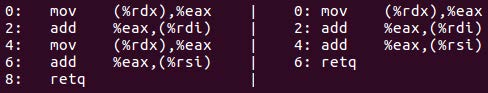
\includegraphics[width=0.9\textwidth]{content/3/chapter10/images/1.jpg}\\
圖10.1 - x86彙編輸出在優化之前(左)和之後(右)
\end{center}

圖10.1展示了GCC為遞增操作生成的x86彙編碼(省略了函數調用和分支,兩種情況下是相同的)。使用別名,編譯器必須從內存中讀取兩次(mov指令)。在手動優化中,只有一次讀取。

這些優化有多重要?其取決於許多因素,所以在沒有進行一些測試之前,不應該著手一個消除代碼中所有的別名。分析器會說明哪些部分是性能熱點,那裡有更多的優化機會。通過為編譯器提供額外的信息,來幫助編譯器的優化通常是最容易實現的(編譯器已經做了最困難的工作)。 

向編譯器提供有關程序的難以發現信息建議的另一方面是,不必擔心編譯器可以很容易地找到的東西。這個問題會在不同的上下文中出現,但更常見的場景是使用函數來驗證輸入。在庫中,有一個用於交換指針的函數:

\begin{lstlisting}[style=styleCXX]
template <typename T>
void my_swap(T* p, T* q) {
	if (p && q) {
		using std::swap;
		swap(*p, *q);
	}
}
\end{lstlisting}

該函數接受空指針,但不對它們做任何操作。在代碼中,由於某種原因,都必須檢查指針,並且只有在兩者都是非空的情況下才調用\texttt{my\_swap()}(如果它們是空的,也許需要做一些其他的事情,所以必須檢查)。忽略其他工作,調用代碼看起來會像這樣:

\begin{lstlisting}[style=styleCXX]
void f(int* p, int* q) {
	if (p && q) my_swap(p, q);
}
\end{lstlisting}

C++開發者花費了過多的時間來爭論冗餘檢查是否會影響性能。我們應該試著刪除調用點的檢查嗎?假設不能,應該創建另一個版本的\texttt{my\_swap()},從而不測試它的輸入嗎?這裡的關鍵是\texttt{my\_swap()}函數是一個模板(和一個小函數),所以肯定會內聯。編譯器擁有所有必要的信息來確定第二個null測試是冗餘的。不是這樣嗎?比較兩個程序的彙編輸出,而不是嘗試對可能的性能差異進行基準測試(在任何情況下,這個差異都是非常小的)。如果編譯器生成的機器代碼有冗餘\texttt{if()}和沒有冗餘\texttt{if()},則可以確定沒有性能差異。下面是GCC在x86上生成的彙編碼:

%\hspace*{\fill} \\ %插入空行
\begin{center}
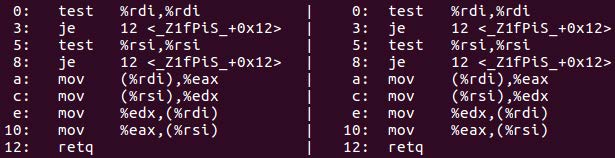
\includegraphics[width=0.9\textwidth]{content/3/chapter10/images/2.jpg}\\
圖10.2 - 有(左)和沒有(右)冗餘指針測試的彙編碼
\end{center}

圖10.2的左邊是為程序生成的兩個\texttt{if()}語句的代碼,一個在\texttt{my\_swap()}中,一個在外部。右邊是\texttt{my\_swap()}的特殊非測試版本的程序代碼。可以看到彙編代碼是完全相同的(如果能夠閱讀x86彙編,還會注意到在這兩種情況下只有兩次比較,而不是四次)。 

內聯在這裡起著至關重要的作用。如果\texttt{my\_swap()}沒有內聯,在函數\texttt{f()}中進行第一次測試是不錯的主意,因為避免了不必要的函數調用,並允許編譯器可以更好地優化,以應對其中一個指針為空的情況。\texttt{my\_swap()}中的測試現在是冗餘的,但編譯器無會生成它,因為它不知道\texttt{my\_swap()}是否在別處調用,可能沒有任何輸入的保證。因為第二次測試是100\%可預測的(在第3章中討論過),所以性能差異幾乎沒有。

這種情況最常見的可能是操作符\texttt{delete},C++允許刪除空指針(什麼都不會發生)。然而,許多開發者仍然這樣寫代碼:

\begin{lstlisting}[style=styleCXX]
if (p) delete p; 
\end{lstlisting}

它是否會影響性能?不會。可以查看彙編輸出,並說服自己,無論是否進行額外檢查,都只對null進行了一次比較。 

現在,已經更好地理解了編譯器如何閱讀程序的。那麼繼續瞭解一種更有用的技術,它可以更好地進行編譯器優化。

\subsubsubsection{10.2.4\hspace{0.2cm}將認知從運行時提升到編譯時}

我們將在這裡討論的方法歸結為,通過將運行時信息轉換為編譯時信息,為編譯器提供有關程序的更多信息。下面的例子中,我們需要處理許多由\textit{Shape}類表示的幾何對象。它們存儲在一個容器中(如果類型是多態的,將是一個指針容器)。該處理包括兩種操作之一:縮小或放大。讓我們來看看代碼:

\hspace*{\fill} \\ %插入空行
\noindent
\textbf{06\_template.C}
\begin{lstlisting}[style=styleCXX]
enum op_t { do_shrink, do_grow };
void process(std::vector<Shape>& v, op_t op) {
	for (Shape& s : v) {
		if (op == do_shrink) s.shrink();
		else s.grow();
	}
}
\end{lstlisting}

概括地說,有一個函數,它的行為在運行時由一個或多個變量控制。通常,這些變量都是布爾型(為了便於閱讀,選擇了枚舉)。如果配置參數\texttt{op}通過引用傳遞,編譯器必須將比較留在循環中,並對每個形狀求值。即使參數是按值傳遞的,許多編譯器也不會將分支提升出循環。需要複製循環體(一個循環用於收縮,一個循環用於增長),編譯器擔心代碼過於膨脹。 

更大的可執行文件需要更長的加載時間,更多的代碼增加了指令緩存的壓力(i-cache,用於緩存即將到來的指令,就像數據緩存即將被CPU使用一樣)。但在某些情況下,這種優化是正確的選擇。通常,會在不更改配置變量的情況下處理大量數據。也許這些變量在整個程序運行過程中都是不變的(只加載一次配置,然後使用)。 

重寫示例,將分支移出循環很容易,但如果代碼很複雜,那麼重構也會很複雜。如果願意來幫助編譯器,可以從編譯器處得到一些幫助。其思想是將運行時值轉換為編譯時值:

\hspace*{\fill} \\ %插入空行
\noindent
\textbf{06\_template.C}
\begin{lstlisting}[style=styleCXX]
template <op_t op>
void process(std::vector<Shape>& v) {
	for (Shape& s : v) {
		if (op == do_shrink) s.shrink();
		else s.grow();
	}
}
void process(std::vector<Shape>& v, op_t op) {
	if (op == do_shrink) process<do_shrink>(v);
	else process<do_grow>(v);
}
\end{lstlisting}

整個(可能很大)舊函數\texttt{process()}轉換為一個模板,除此之外,沒有任何變化,沒有將分支移出循環。但是,控制該分支的條件現在是一個編譯時常量(模板參數),編譯器會在每個模板實例化中消除分支和相應的固定代碼。在程序的其餘部分,配置變量仍然是一個運行時值,只是一個不經常更改(或根本不更改)的值罷了。因此,仍然需要一個運行時測試,但它僅用於決定調用哪個實例化的模板。

這種方法可以推廣。假設需要計算每個形狀的一些屬性,比如體積、尺寸、重量等。這都可以由一個函數完成,因為許多計算可以在不同的屬性之間共享。但需要時間來計算不需要的屬性,所以可以實現這樣的函數:

\begin{lstlisting}[style=styleCXX]
void measure(const std::vector<Shape>& s,
	double* length, double* width, double* depth,
	double* volume, double* weight);
\end{lstlisting}

空指針是有效的,表示不需要這個結果。在函數內部為請求值的特定組合編寫最優的代碼,只執行一次普通的計算。然而,這種檢查是在循環中對形狀進行的,這一次是一組相當複雜的條件。如果需要為同一組度量處理許多種形狀,需要將條件提升到循環之外是有意義的,但編譯器不太可能這樣做(即使它可以)。同樣,可以編寫帶有許多非類型形參的模板(它們將是布爾值),如\texttt{need\_length},\texttt{need\_width}等。在該模板內部,因為現在這是編譯時信息,編譯器將消除所有從未執行的分支。在運行時調用的函數必須根據指針是否為空,將數據調用或轉發到正確的模板實例化。最有效的實現方式是查找表:

\hspace*{\fill} \\ %插入空行
\noindent
\textbf{07\_measure.C}
\begin{lstlisting}[style=styleCXX]
template <bool use_length, bool use_width, …>
void measure(const std::vector<Shape>& v,
double* length, … );
void measure(const std::vector<Shape>& v,
double* length, … ) {
	const int key = ((length != nullptr) << 0) |
					((width  != nullptr) << 1) |
				    ((depth  != nullptr) << 2) |
				    ((volume != nullptr) << 3) |
				    ((weight != nullptr) << 4);
	switch (key) {
		case 0x01: measure<true , false, … >(v, length, … );
		break;
		case 0x02: measure<false, true , … >(v, length, … );
		break;
		…
		default:; // Programming error, assert
	}
}
\end{lstlisting}

這將生成大量代碼,測試的每個變體都是一個新函數。這樣轉換的效果應該通過分析來驗證,但在測試相對簡單的情況下(例如,許多形狀都是一個立方體),並且對許多(數百萬)形狀請求相同的測試集時,這種修改可以獲得更可觀的性能收益。 

使用特定的編譯器時,瞭解編譯器的功能(包括優化)很有用。這樣的詳細程度超出了本書的範圍,而且這是一種易變的知識——編譯器發展得很快。相反,本章為理解編譯器優化奠定了基礎,併為讀者提供了參考框架。


